\documentclass[tikz, border=10pt]{standalone}
% Shared preamble — % Shared preamble — % Shared preamble — \input{preamble} in each figure file.
% Compiled via Makefile which sets TEXINPUTS so this file is always found.

% -----------------------------------------------------------------------
% Fonts — matches ntnuthesis.cls
% -----------------------------------------------------------------------
\usepackage[utf8]{inputenc}
\usepackage[T1]{fontenc}
\usepackage[charter, cal=cmcal]{mathdesign} % Charter body + math font
\usepackage[scaled=.88]{berasans}           % Bera sans-serif
\usepackage[scaled=.82]{DejaVuSansMono}     % DejaVu monospace (for \texttt)

% -----------------------------------------------------------------------
% TikZ & PGF
% -----------------------------------------------------------------------
\usepackage{tikz}
\usetikzlibrary{
  positioning,
  arrows.meta,
  fit,
  calc,
  backgrounds,
  shapes.geometric,
  shapes.multipart,
  shapes.symbols,
  shapes.callouts,
  shapes.arrows,
  shapes.misc,
  decorations.pathreplacing,
  decorations.markings,
  matrix,
}
\usepackage{pgf-umlsd}
\usepackage{pgfplots}
\usepackage{pgfplotstable}
\pgfplotsset{compat=1.18}
\usepgfplotslibrary{fillbetween}

% -----------------------------------------------------------------------
% Math
% -----------------------------------------------------------------------
\usepackage{amsmath}

% -----------------------------------------------------------------------
% Color palette
% -----------------------------------------------------------------------
% Semantic NLP / model-diagram colors
\colorlet{tok}{green!35!black}
\colorlet{emb}{yellow!70!orange}
\colorlet{trm}{blue!55!black}
\colorlet{out}{red!70!black}
% General purpose
\colorlet{clrA}{blue!60!black}
\colorlet{clrB}{orange!80!black}
\colorlet{clrC}{green!50!black}
\colorlet{clrD}{red!65!black}
\colorlet{clrE}{violet!70!black}
% Neutral fills
\colorlet{fillLight}{gray!12}
\colorlet{fillMed}{gray!25}

% -----------------------------------------------------------------------
% Global TikZ styles
% NOTE: no blank lines inside \tikzset{} — blank lines produce \par and
%       break pgfkeys parsing.
% -----------------------------------------------------------------------
\tikzset{
  >=Latex,
  % --- generic boxes ---
  box/.style={rectangle, draw, thick, align=center, inner sep=4pt, minimum height=8mm},
  rbox/.style={box, rounded corners=6pt},
  dbox/.style={box, dashed},
  % --- NLP diagram node types ---
  token/.style={rbox, draw=tok!80, fill=tok!20, minimum width=1.8cm, font=\small},
  embed/.style={box, draw=emb!90, fill=emb!30, minimum width=1.4cm},
  trm/.style={ellipse, draw=trm!90, fill=trm!20, minimum width=1.6cm, minimum height=8mm},
  output/.style={rbox, draw=out!90, fill=out!20, minimum width=1.7cm, font=\small},
  % --- arrows ---
  arrow/.style={-{Stealth[length=2mm]}, thick},
  connect/.style={->, thick, gray!65},
  darrow/.style={<->, thick},
  % --- annotation ---
  labelbox/.style={draw, thick, inner sep=4pt, rounded corners=3pt, font=\scriptsize\bfseries},
}
 in each figure file.
% Compiled via Makefile which sets TEXINPUTS so this file is always found.

% -----------------------------------------------------------------------
% Fonts — matches ntnuthesis.cls
% -----------------------------------------------------------------------
\usepackage[utf8]{inputenc}
\usepackage[T1]{fontenc}
\usepackage[charter, cal=cmcal]{mathdesign} % Charter body + math font
\usepackage[scaled=.88]{berasans}           % Bera sans-serif
\usepackage[scaled=.82]{DejaVuSansMono}     % DejaVu monospace (for \texttt)

% -----------------------------------------------------------------------
% TikZ & PGF
% -----------------------------------------------------------------------
\usepackage{tikz}
\usetikzlibrary{
  positioning,
  arrows.meta,
  fit,
  calc,
  backgrounds,
  shapes.geometric,
  shapes.multipart,
  shapes.symbols,
  shapes.callouts,
  shapes.arrows,
  shapes.misc,
  decorations.pathreplacing,
  decorations.markings,
  matrix,
}
\usepackage{pgf-umlsd}
\usepackage{pgfplots}
\usepackage{pgfplotstable}
\pgfplotsset{compat=1.18}
\usepgfplotslibrary{fillbetween}

% -----------------------------------------------------------------------
% Math
% -----------------------------------------------------------------------
\usepackage{amsmath}

% -----------------------------------------------------------------------
% Color palette
% -----------------------------------------------------------------------
% Semantic NLP / model-diagram colors
\colorlet{tok}{green!35!black}
\colorlet{emb}{yellow!70!orange}
\colorlet{trm}{blue!55!black}
\colorlet{out}{red!70!black}
% General purpose
\colorlet{clrA}{blue!60!black}
\colorlet{clrB}{orange!80!black}
\colorlet{clrC}{green!50!black}
\colorlet{clrD}{red!65!black}
\colorlet{clrE}{violet!70!black}
% Neutral fills
\colorlet{fillLight}{gray!12}
\colorlet{fillMed}{gray!25}

% -----------------------------------------------------------------------
% Global TikZ styles
% NOTE: no blank lines inside \tikzset{} — blank lines produce \par and
%       break pgfkeys parsing.
% -----------------------------------------------------------------------
\tikzset{
  >=Latex,
  % --- generic boxes ---
  box/.style={rectangle, draw, thick, align=center, inner sep=4pt, minimum height=8mm},
  rbox/.style={box, rounded corners=6pt},
  dbox/.style={box, dashed},
  % --- NLP diagram node types ---
  token/.style={rbox, draw=tok!80, fill=tok!20, minimum width=1.8cm, font=\small},
  embed/.style={box, draw=emb!90, fill=emb!30, minimum width=1.4cm},
  trm/.style={ellipse, draw=trm!90, fill=trm!20, minimum width=1.6cm, minimum height=8mm},
  output/.style={rbox, draw=out!90, fill=out!20, minimum width=1.7cm, font=\small},
  % --- arrows ---
  arrow/.style={-{Stealth[length=2mm]}, thick},
  connect/.style={->, thick, gray!65},
  darrow/.style={<->, thick},
  % --- annotation ---
  labelbox/.style={draw, thick, inner sep=4pt, rounded corners=3pt, font=\scriptsize\bfseries},
}
 in each figure file.
% Compiled via Makefile which sets TEXINPUTS so this file is always found.

% -----------------------------------------------------------------------
% Fonts — matches ntnuthesis.cls
% -----------------------------------------------------------------------
\usepackage[utf8]{inputenc}
\usepackage[T1]{fontenc}
\usepackage[charter, cal=cmcal]{mathdesign} % Charter body + math font
\usepackage[scaled=.88]{berasans}           % Bera sans-serif
\usepackage[scaled=.82]{DejaVuSansMono}     % DejaVu monospace (for \texttt)

% -----------------------------------------------------------------------
% TikZ & PGF
% -----------------------------------------------------------------------
\usepackage{tikz}
\usetikzlibrary{
  positioning,
  arrows.meta,
  fit,
  calc,
  backgrounds,
  shapes.geometric,
  shapes.multipart,
  shapes.symbols,
  shapes.callouts,
  shapes.arrows,
  shapes.misc,
  decorations.pathreplacing,
  decorations.markings,
  matrix,
}
\usepackage{pgf-umlsd}
\usepackage{pgfplots}
\usepackage{pgfplotstable}
\pgfplotsset{compat=1.18}
\usepgfplotslibrary{fillbetween}

% -----------------------------------------------------------------------
% Math
% -----------------------------------------------------------------------
\usepackage{amsmath}

% -----------------------------------------------------------------------
% Color palette
% -----------------------------------------------------------------------
% Semantic NLP / model-diagram colors
\colorlet{tok}{green!35!black}
\colorlet{emb}{yellow!70!orange}
\colorlet{trm}{blue!55!black}
\colorlet{out}{red!70!black}
% General purpose
\colorlet{clrA}{blue!60!black}
\colorlet{clrB}{orange!80!black}
\colorlet{clrC}{green!50!black}
\colorlet{clrD}{red!65!black}
\colorlet{clrE}{violet!70!black}
% Neutral fills
\colorlet{fillLight}{gray!12}
\colorlet{fillMed}{gray!25}

% -----------------------------------------------------------------------
% Global TikZ styles
% NOTE: no blank lines inside \tikzset{} — blank lines produce \par and
%       break pgfkeys parsing.
% -----------------------------------------------------------------------
\tikzset{
  >=Latex,
  % --- generic boxes ---
  box/.style={rectangle, draw, thick, align=center, inner sep=4pt, minimum height=8mm},
  rbox/.style={box, rounded corners=6pt},
  dbox/.style={box, dashed},
  % --- NLP diagram node types ---
  token/.style={rbox, draw=tok!80, fill=tok!20, minimum width=1.8cm, font=\small},
  embed/.style={box, draw=emb!90, fill=emb!30, minimum width=1.4cm},
  trm/.style={ellipse, draw=trm!90, fill=trm!20, minimum width=1.6cm, minimum height=8mm},
  output/.style={rbox, draw=out!90, fill=out!20, minimum width=1.7cm, font=\small},
  % --- arrows ---
  arrow/.style={-{Stealth[length=2mm]}, thick},
  connect/.style={->, thick, gray!65},
  darrow/.style={<->, thick},
  % --- annotation ---
  labelbox/.style={draw, thick, inner sep=4pt, rounded corners=3pt, font=\scriptsize\bfseries},
}


\begin{document}
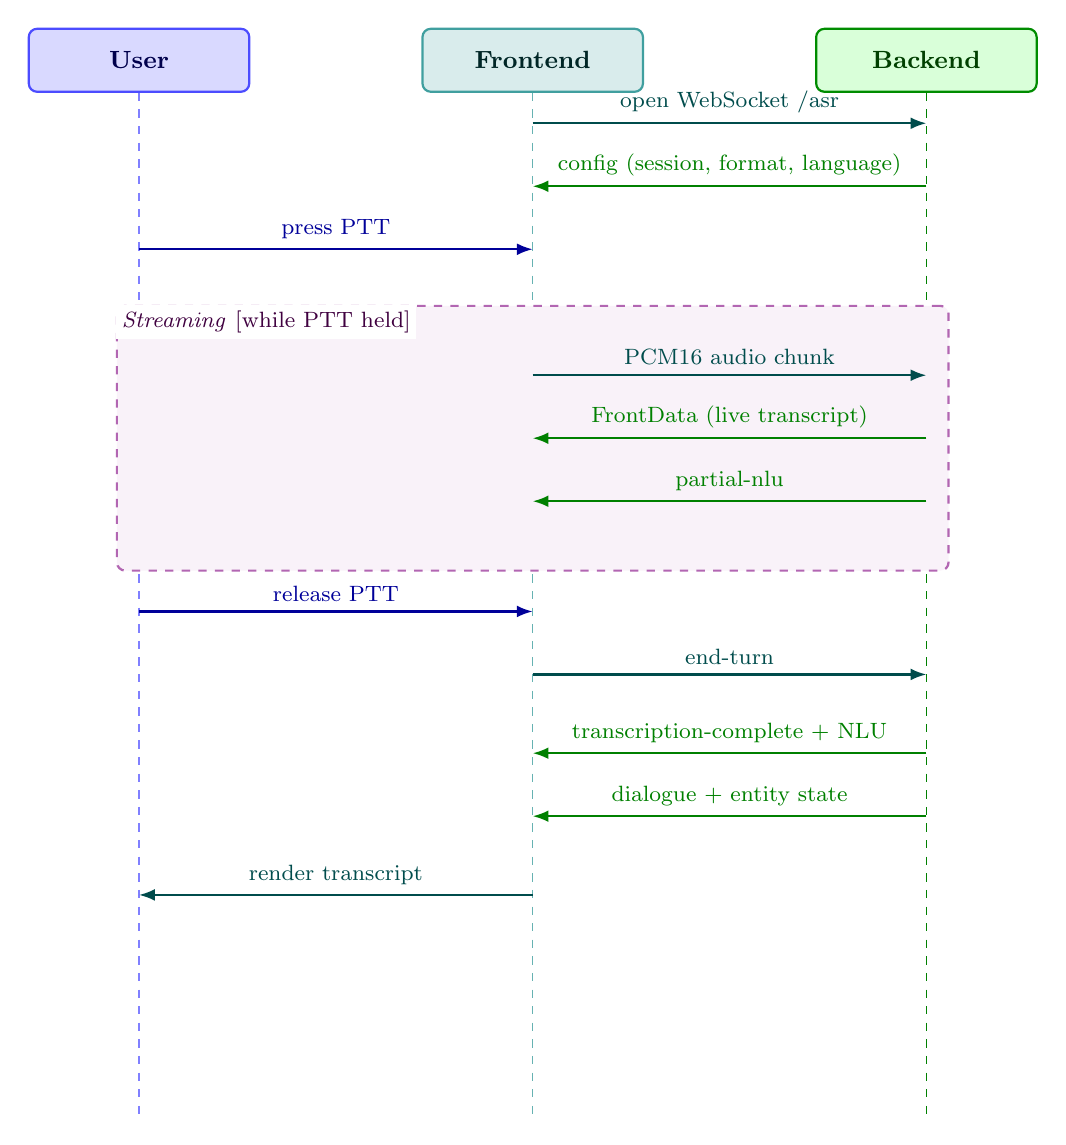
\begin{tikzpicture}[
    font=\small\sffamily,
    useractor/.style={
        draw=blue!70, thick, rounded corners=3pt,
        minimum width=2.8cm, minimum height=0.8cm,
        fill=blue!15, align=center, font=\small\bfseries,
        text=blue!30!black
    },
    frontactor/.style={
        draw=teal!75, thick, rounded corners=3pt,
        minimum width=2.8cm, minimum height=0.8cm,
        fill=teal!15, align=center, font=\small\bfseries,
        text=teal!30!black
    },
    backactor/.style={
        draw=green!55!black, thick, rounded corners=3pt,
        minimum width=2.8cm, minimum height=0.8cm,
        fill=green!15, align=center, font=\small\bfseries,
        text=green!25!black
    },
    msg/.style={-{Latex[length=2mm]}, thick, #1},
    msg/.default=black!70,
    msglabel/.style={font=\footnotesize, midway, above, align=center},
    block/.style={
        draw=violet!60, dashed, rounded corners=3pt,
        inner sep=8pt, fill=violet!5, thick
    },
    blocklabel/.style={
        font=\footnotesize\itshape, fill=white,
        inner sep=2pt, anchor=north west,
        text=violet!50!black
    },
]

    %% ── Lifelines (top boxes) ───────────────────────────────
    \node[useractor]  (user)     at (0, 0)  {User};
    \node[frontactor] (frontend) at (5, 0)  {Frontend};
    \node[backactor]  (backend)  at (10, 0) {Backend};

    %% ── Lifeline columns (vertical dashed) ──────────────────
    \draw[dashed, blue!50]      (user.south)     -- ($(user.south)     + (0,-13)$);
    \draw[dashed, teal!60]      (frontend.south) -- ($(frontend.south) + (0,-13)$);
    \draw[dashed, green!50!black] (backend.south)  -- ($(backend.south)  + (0,-13)$);

    %% ── Y-coordinates for messages ──────────────────────────
    \def\ya{-0.8}    % open WebSocket
    \def\yb{-1.6}    % config
    \def\yc{-2.4}    % press PTT
    \def\yd{-3.4}    % streaming block top
    \def\ye{-4.0}    %   PCM16 chunk
    \def\yf{-4.8}    %   FrontData
    \def\yg{-5.6}    %   partial-nlu
    \def\yh{-6.2}    % streaming block bottom
    \def\yi{-7.0}    % release PTT
    \def\yj{-7.8}    % end-turn
    \def\yk{-8.8}    % transcription-complete
    \def\yl{-9.6}    % dialogue
    \def\ym{-10.6}   % render to user

    %% ── Setup phase ─────────────────────────────────────────
    \draw[msg=teal!60!black] (frontend |- 0,\ya) -- node[msglabel] {open WebSocket /asr}
               (backend  |- 0,\ya);
    \draw[msg=green!50!black] (backend  |- 0,\yb) -- node[msglabel] {config (session, format, language)}
               (frontend |- 0,\yb);

    %% ── User starts ─────────────────────────────────────────
    \draw[msg=blue!60!black] (user     |- 0,\yc) -- node[msglabel] {press PTT}
               (frontend |- 0,\yc);

    %% ── Streaming block ─────────────────────────────────────
    \node[block, fit={(user |- 0,\yd) (backend |- 0,\yh)}] (stream) {};
    \node[blocklabel] at (stream.north west) {Streaming \textnormal{[while PTT held]}};

    \draw[msg=teal!60!black] (frontend |- 0,\ye) -- node[msglabel] {PCM16 audio chunk}
               (backend  |- 0,\ye);
    \draw[msg=green!50!black] (backend  |- 0,\yf) -- node[msglabel] {FrontData (live transcript)}
               (frontend |- 0,\yf);
    \draw[msg=green!50!black] (backend  |- 0,\yg) -- node[msglabel] {partial-nlu}
               (frontend |- 0,\yg);

    %% ── User releases ───────────────────────────────────────
    \draw[msg=blue!60!black] (user     |- 0,\yi) -- node[msglabel] {release PTT}
               (frontend |- 0,\yi);
    \draw[msg=teal!60!black] (frontend |- 0,\yj) -- node[msglabel] {end-turn}
               (backend  |- 0,\yj);

    %% ── Final results ───────────────────────────────────────
    \draw[msg=green!50!black] (backend  |- 0,\yk) -- node[msglabel] {transcription-complete + NLU}
               (frontend |- 0,\yk);
    \draw[msg=green!50!black] (backend  |- 0,\yl) -- node[msglabel] {dialogue + entity state}
               (frontend |- 0,\yl);

    %% ── Display ─────────────────────────────────────────────
    \draw[msg=teal!60!black] (frontend |- 0,\ym) -- node[msglabel] {render transcript}
               (user     |- 0,\ym);

\end{tikzpicture}
\end{document}
